\documentclass[aspectratio=169]{beamer}
\usetheme{Madrid}
\usecolortheme{default}

\usepackage[utf8]{inputenc}
\usepackage[T1]{fontenc}
\usepackage{tikz}
\usepackage{hyperref}
\usepackage{fontawesome5}

\usetikzlibrary{shapes.geometric, arrows, positioning, shadows}

\definecolor{kivablue}{RGB}{41,128,185}
\definecolor{kivagreen}{RGB}{39,174,96}
\definecolor{kivaorange}{RGB}{230,126,34}
\definecolor{kivared}{RGB}{231,76,60}
\definecolor{kivagray}{RGB}{127,140,141}

\setbeamercolor{structure}{fg=kivablue}
\setbeamercolor{palette primary}{bg=kivablue,fg=white}
\setbeamercolor{palette secondary}{bg=kivagreen,fg=white}
\setbeamercolor{palette tertiary}{bg=kivaorange,fg=white}

\title[KIVA Deploy]{Deploying KIVA on Your Machine}
\subtitle{A Quick Walkthrough}
\author{MA AI Hub x SundAI Pre-Session}
\date{May 6, 2026}

\begin{document}

\begin{frame}
\titlepage
\end{frame}

\begin{frame}{About KIVA}
\begin{center}
\Large KIVA is built on \textbf{Riverst}
\end{center}

\vspace{0.5cm}

\begin{block}{Original Project}
\textbf{Riverst} by Sensein Lab\\
\small
\url{https://github.com/sensein/riverst}\\[0.2cm]
Platform for building interactive user-avatar conversations with speech analysis
\end{block}

\vspace{0.3cm}

\begin{block}{This Fork}
\textbf{KIVA} (Knowledge Integration and Vocabulary Acquisition)\\
\small
\url{https://github.com/ebaenamar/KIVA}\\[0.2cm]
Adds easy installation scripts and deployment guides for educational activities
\end{block}

\vspace{0.3cm}

\begin{center}
\textcolor{kivagray}{\small This presentation uses the KIVA fork for simplified setup}
\end{center}
\end{frame}

\begin{frame}{What You Need}
\begin{columns}[T]
\column{0.5\textwidth}
\textbf{Hardware \& OS}
\begin{itemize}
    \item macOS (Apple Silicon) or Ubuntu Linux
    \item \textcolor{kivaorange}{Windows:} Use GitHub Codespaces
\end{itemize}

\vspace{0.5cm}
\textbf{Software}
\begin{itemize}
    \item Python 3.11+ (or conda)
    \item Node.js 16+
    \item Git
    \item Chrome 134+ (for WebRTC)
\end{itemize}

\column{0.5\textwidth}
\textbf{API Keys}
\begin{itemize}
    \item \textbf{Required:} OpenAI API key
    \item \textbf{Optional:} Hugging Face token
\end{itemize}

\vspace{0.3cm}
\begin{block}{Get your OpenAI key}
\small
\url{https://platform.openai.com/api-keys}
\end{block}

\vspace{0.3cm}
\begin{alertblock}{Windows Users}
\small See slide on GitHub Codespaces
\end{alertblock}
\end{columns}
\end{frame}

\begin{frame}{Step 1: Clone the Repo}
\begin{center}
\Large \texttt{git clone https://github.com/ebaenamar/KIVA.git}
\end{center}

\vspace{0.5cm}
\begin{center}
\large \texttt{cd KIVA}
\end{center}

\vspace{0.8cm}
\begin{block}{What you get}
\texttt{src/server/} -- Python backend \quad \textbar\quad \texttt{src/client/react/} -- React frontend
\end{block}
\end{frame}

\begin{frame}{Step 2: Server Setup}
\textbf{Create a conda environment and install dependencies:}

\vspace{0.3cm}

\begin{tabular}{@{}l@{\hspace{0.5cm}}l@{}}
\texttt{cd src/server} & \\
\texttt{conda create -n riverst python=3.11} & \textcolor{kivagreen}{\faCheck\ one-time only} \\
\texttt{conda activate riverst} & \textcolor{kivablue}{\faSync\ every time} \\
\texttt{conda install -c conda-forge ffmpeg} & \textcolor{kivagreen}{\faCheck\ one-time only} \\
\texttt{pip install -r requirements.txt} & \textcolor{kivagreen}{\faCheck\ one-time only} \\
\end{tabular}

\vspace{0.5cm}

\begin{alertblock}{No conda?}
Use \texttt{venv} instead: \texttt{python -m venv venv \&\& source venv/bin/activate}
Install ffmpeg via your system package manager, then \texttt{pip install -r requirements.txt}
\end{alertblock}
\end{frame}

\begin{frame}{Step 3: Configure Environment}
\textbf{Server} (\texttt{src/server/.env}):
\begin{enumerate}
    \item \texttt{cp env.example .env}
    \item Open \texttt{.env} and set:
    \begin{itemize}
        \item \texttt{OPENAI\_API\_KEY="sk-your-key-here"} \textcolor{kivared}{\faExclamationCircle\ required}
        \item \texttt{HF\_TOKEN="hf\_..."} \textcolor{kivagray}{optional}
        \item Leave everything else as-is
    \end{itemize}
\end{enumerate}

\vspace{0.3cm}

\textbf{Client} (\texttt{src/client/react/.env}):
\begin{enumerate}
    \item \texttt{cp env.example .env}
    \item Change \texttt{VITE\_API\_PROXY\_TARGET} to \texttt{http://localhost:7860}
    \item Leave everything else as-is
\end{enumerate}
\end{frame}

\begin{frame}{Step 4: Client Setup}
\begin{center}
\LARGE \texttt{cd src/client/react}
\end{center}

\vspace{0.3cm}

\begin{center}
\LARGE \texttt{npm install}
\end{center}

\vspace{0.5cm}

\begin{block}{One command, that's it.}
Node handles everything via \texttt{package.json}.
\end{block}
\end{frame}

\begin{frame}{Step 5 of 5: Start KIVA!}
\textbf{Option A: Automatic (recommended)} -- Use the helper scripts:

\vspace{0.2cm}

\begin{columns}[T]
\column{0.5\textwidth}
\begin{block}{Terminal 1}
\small
\texttt{cd riverst}\\
\texttt{./start\_server.sh}\\[0.2cm]
\textcolor{kivagray}{\footnotesize Handles everything automatically}
\end{block}

\column{0.5\textwidth}
\begin{block}{Terminal 2}
\small
\texttt{cd riverst}\\
\texttt{./start\_client.sh}\\[0.2cm]
\textcolor{kivagray}{\footnotesize Checks server is running first}
\end{block}
\end{columns}

\vspace{0.3cm}

\textbf{Option B: Manual} -- Run commands yourself:

\vspace{0.1cm}

\begin{columns}[T]
\column{0.5\textwidth}
\begin{block}{Terminal 1}
\footnotesize
\texttt{cd riverst/src/server}\\
\texttt{conda activate riverst}\\
\texttt{python main.py}
\end{block}

\column{0.5\textwidth}
\begin{block}{Terminal 2}
\footnotesize
\texttt{cd riverst/src/client/react}\\
\texttt{npm run dev}
\end{block}
\end{columns}

\vspace{0.2cm}

\begin{center}
\large Open Chrome: \texttt{http://localhost:5173}
\end{center}
\end{frame}

\begin{frame}{Step 6: Select an Avatar and Go}
\begin{enumerate}
    \setlength\itemsep{0.5cm}
    \item On the homepage, click \textbf{``Select your avatar''}
    \item Click on \textbf{Fabio} or \textbf{Bruce}
    \item Go back to the homepage
    \item Under \textbf{``Playground''}, click \textbf{``Demo ready to go''}
    \item Click \textbf{``Run a demo''}
    \item Allow microphone access when prompted
    \item Start talking to your avatar!
\end{enumerate}
\end{frame}

\begin{frame}{Troubleshooting}
\begin{itemize}
    \setlength\itemsep{0.4cm}
    \item \textbf{``Failed to create session''} -- Check OpenAI key in \texttt{src/server/.env}
    \item \textbf{Avatar not loading} -- Clear browser cache or reset avatar in console
    \item \textbf{No microphone access} -- Check Chrome permissions (Settings $\rightarrow$ Privacy $\rightarrow$ Microphone)
    \item \textbf{Port already in use} -- Kill existing processes: \texttt{lsof -i :7860} or \texttt{lsof -i :5173}
    \item \textbf{ffmpeg not found} -- \texttt{conda install -c conda-forge ffmpeg} or \texttt{brew install ffmpeg}
    \item \textbf{npm install fails} -- Try \texttt{rm -rf node\_modules \&\& npm install}
\end{itemize}
\end{frame}

\begin{frame}{Windows Users: GitHub Codespaces}
\small
\textbf{KIVA doesn't run natively on Windows.} Use GitHub Codespaces:

\vspace{0.2cm}

\begin{enumerate}
    \setlength\itemsep{0.25cm}
    \item Go to \texttt{https://github.com/ebaenamar/KIVA}
    \item Click green \textbf{Code} button $\rightarrow$ \textbf{Codespaces} tab
    \item Click \textbf{Create codespace on main} (wait 2-3 min)
    \item In terminal: \texttt{./start\_server.sh} (Terminal 1)
    \item New terminal: \texttt{./start\_client.sh} (Terminal 2)
    \item \textbf{Ports} tab $\rightarrow$ forward port 5173
    \item Open the forwarded URL in browser
\end{enumerate}

\vspace{0.3cm}

\begin{columns}[T]
\column{0.5\textwidth}
\begin{block}{Free tier}
\footnotesize
60 hrs/month free
\end{block}

\column{0.5\textwidth}
\begin{alertblock}{API Key}
\footnotesize
Set in \texttt{src/server/.env}
\end{alertblock}
\end{columns}
\end{frame}

\begin{frame}{Quick Reference Card}
\begin{center}
\begin{tikzpicture}[
    node distance=0.8cm,
    stepbox/.style={rectangle, rounded corners, draw=kivablue, fill=kivablue!15, thick, minimum width=9cm, minimum height=0.7cm, align=center, font=\small},
    arr/.style={->, >=stealth, thick, color=kivablue}
]

\node[stepbox] (s1) {\faGithub\ \texttt{git clone https://github.com/ebaenamar/KIVA.git}};
\node[stepbox, below=of s1] (s2) {\faKey\ \texttt{cd KIVA/src/server \&\& cp env.example .env} -- Add OpenAI key};
\node[stepbox, below=of s2] (s3) {\faPlay\ \texttt{./start\_server.sh} (Terminal 1)};
\node[stepbox, below=of s3] (s4) {\faPlay\ \texttt{./start\_client.sh} (Terminal 2)};
\node[stepbox, below=of s4] (s5) {\faChrome\ Open \texttt{http://localhost:5173} in Chrome};

\draw[arr] (s1) -- (s2);
\draw[arr] (s2) -- (s3);
\draw[arr] (s3) -- (s4);
\draw[arr] (s4) -- (s5);

\end{tikzpicture}
\end{center}
\end{frame}

\begin{frame}
\begin{center}
\vspace{1cm}
\Huge That's it!

\vspace{1cm}

\Large Questions?

\vspace{1cm}

\normalsize
\faGithub\ \url{https://github.com/sensein/riverst}

\vspace{0.3cm}

\faEnvelope\ Reach out on Slack if you get stuck
\end{center}
\end{frame}

\end{document}
